\documentclass[10pt,portuguese]{article}
\usepackage[portuguese]{babel}

\usepackage{fourier}
\usepackage[bottom]{footmisc}

\usepackage[]{graphicx}
\usepackage[]{color}
\usepackage{xcolor}
\usepackage{alltt}
\usepackage{listings}
\usepackage[T1]{fontenc}
\usepackage[utf8]{inputenc}
\setlength{\parskip}{\smallskipamount}
\setlength{\parindent}{5ex}
\usepackage{indentfirst}
\usepackage{listings}
\usepackage{setspace}
\usepackage{hyperref}
\hypersetup{
    colorlinks=true,
    linkcolor=auburn,
    filecolor=magenta,      
    urlcolor=blue, urlsize=2em
}

% Set page margins
\usepackage[top=100pt,bottom=100pt,left=68pt,right=66pt]{geometry}

% Package used for placeholder text
\usepackage{lipsum}

% Prevents LaTeX from filling out a page to the bottom
\raggedbottom


\usepackage{fancyhdr}
\fancyhf{} 
\fancyfoot[C]{\thepage}
\renewcommand{\headrulewidth}{0pt} 
\pagestyle{fancy}

\usepackage{titlesec}
\titleformat{\chapter}
   {\normalfont\LARGE\bfseries}{\thechapter.}{1em}{}
\titlespacing{\chapter}{0pt}{50pt}{2\baselineskip}

\usepackage{float}
\floatstyle{plaintop}
\restylefloat{table}

\usepackage[tableposition=top]{caption}


\definecolor{light-gray}{gray}{0.95}

\renewcommand{\contentsname}{Índice}

\begin{document}


\begin{titlepage}
	\clearpage\thispagestyle{empty}
	\centering
	\vspace{2cm}

	
	{\Large  Padrões e Desenho de Software \par}
	\vspace{0.5cm}
	{\small Professor: \\
	José Luis Oliveira\par
	Sérgio Matos\par}
	\vspace{4cm}
	{ \textbf{Padrões de desenho de Software:}} \\
	\vspace{0.5cm}
	{\Huge \textbf{Composite \& Command}} \\
	\vspace{1cm}
	\vspace{4cm}
	{\normalsize  Hugo Paiva, 93195
	   \par}
	 
	\vspace{2cm}

    
\includegraphics[scale=0.20]{logo_ua.png}
    
    \vspace{2cm}
    
	{\normalsize DETI \\ 
		Universidade de Aveiro \par}
		
	{\normalsize 05-06-2020 \par}
	\vspace{2cm}
		
	
	\pagebreak

\end{titlepage}
\tableofcontents{}
\clearpage

\section{Composite}
\subsection{Descrição}
\par \textit{Composite} pertence aos padrões de desenho de software estrutural, dando, portanto, conselhos relacionados com a composição de classes e/ou objetos.

\par Todos os problemas que podem ser modelados em estruturas de árvore são potenciais candidatos para este padrão de software no entanto, \textit{Composite} resolve especialmente os problemas em que um objeto composto é manipulado de forma diferente que um objeto singular, evitando verificações ou qualquer outro tipo de mecanismo para selecionar diferentes implementações entre estes dois tipos de objetos. Em suma, independentemente do tipo de objeto, usando este padrão, deve-se poder tratá-lo de igual forma.

\begin{figure}[!h]
    \centering
    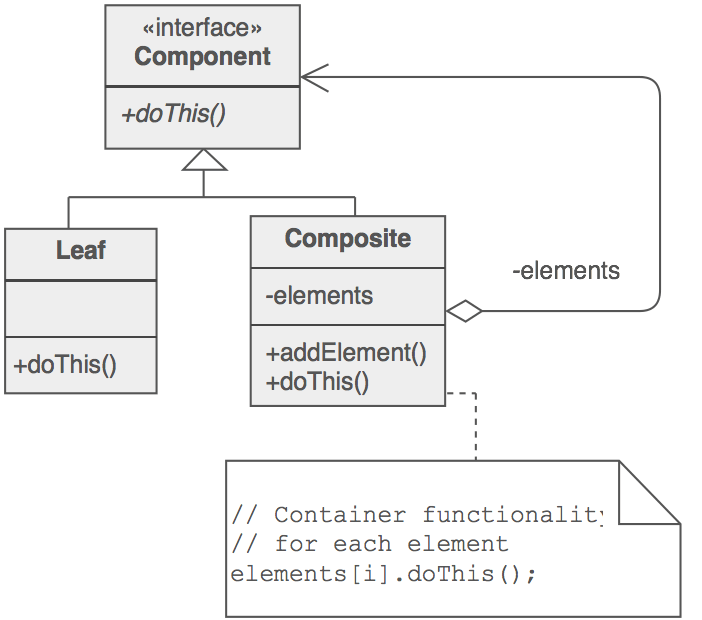
\includegraphics[width=200]{images/composite/UML.png}
    \caption{Estrutura usual do padrão \textit{Composite} em um diagrama de classes}
\end{figure}

\par Como é possível observar a partir da Figura 1, independentemente do tipo de objeto, ambos implementam o mesmo método, permitindo, no entanto,  a adição de outros objetos no objeto composto. De notar que, apesar do método ter o mesmo nome, apresentando transparência e facilidade ao cliente, dependendo do tipo do objeto, a implementação é diferente, sendo usual percorrer o filhos e chamar o mesmo método no objeto composto, como é possível observar na Figura.

\par Existem, no entanto, outros tipo de implementações ao utilizar este padrão com a possibilidade de permitir a remoção de objetos contidos no objeto composto ou, por exemplo, permitir apenas a substituição dos objetos guardados, por um novo, ao invés de adicionar, com o benefício da melhor compreensão do programa, mas reduzindo a flexibilidade. Dito isto, todas estas pequenas modificações sugeridas ao exemplo da Figura 1 continuam a manter a base do padrão \textit{Composite}, sendo totalmente válidas.


\par 

\par 
\subsection{Problema}
\subsection{Solução}

\clearpage

\section{Command}
\subsection{Descrição}

\par É expectável que um padrão de desenho de software comportamental, para além de fornecer boas práticas para resolver um determinado problema, foque as mesmas na forma como as classes e objetos interagem e distribuem responsabilidades.\textit{Command}, sendo um destes tipos de padrões, foca-se exactamente nesse ponto.

\par O problema que este padrão resolve incide não só na repetição de código mas também na organização geral das classes e das responsabilidades. Seguindo o \textit{Single Responsibility Principle} e \textit{Open/Closed Principle}, este padrão separa a entidade que invoca uma ação, da entidade que a executa, colocando uma entidade intermédia, o \textit{Command}, que é responsável por chamar o método que desempenha a ação na entidade receptora, tal como o primeiro principio citado o dita.
Ao fazer isto, são evitados os problemas de repetição de código, pois a entidade intermédia pode ser reutilizada múltiplas vezes, bem como problemas relacionados com limitações de comandos ou de alterações às outras entidades, de acordo com o segundo principio citado.

\par No fundo, está-se a encapsular um pedido num objeto, criando a possibilidade de adicionar mais métodos ao objeto criado, complementares à simples ação pedida pelo cliente.
A aproximação mais usual é a adição de um método que permite reverter o comando no entanto, o céu é o limite, podemos criar métodos que permitem adicionar um simples atraso à operação, até à execução de múltiplos comandos com apenas um pedido.





\par EXEMPLOS

\par

Considerando, por exemplo, um comando de televisão, este executa múltiplas ações sobre uma televisão, repetindo as ações ao longo da sua utilização. Aproximando este exemplo a uma linguagem de programação, não faria sentido, sempre que um determinado botão fosse clicado, criar um novo objeto com um determinado método ou até mesmo executar um código repetidamente, que apenas funcionaria para uma televisão em específico. 
Seguindo a lógica do \textit{Command}, faz muito mais sentido instanciar uma classe que armazena a televisão recetora do pedido e que, daí em diante, apenas necessita que lhe chamem o seu método específico para executar a ação, reutilizando e uniformizando o código. 

 Um dos exemplo mais banais desta situação é toda a gestão que um programa ou sistema operativo faz dos \textit{inputs} de um utilizador. 
Ao utilizar, por exemplo, qualquer tipo de editor de texto, o sistema operativo permite ao utilizador inserir caracteres num campo mas, permite, também, reverter essas inserções (com a ajuda do atalho \textit{ctrl+z}). Ora, isto é um exemplo visível onde faria sentido aplicar este padrão de desenho de software.

\par Pessoalmente, sendo eu um utilizador casual de algum software de edição de imagens e vídeo (\textit{Adobe Photoshop, Adobe Illustrator e Final Cut Pro}), ao associar o \textit{Command} à gestão que estes programas fazem das ações dos utilizadores, os conceitos análogos ao mesmo tornaram-se ainda mais claros. Pegando no exemplo do \textit{Adobe Photoshop}, todas as alterações que são feitas a uma imagem podem ser desfeitas múltiplas vezes, tanto pela mesma ordem em que foram executadas, como também voltar a refazê-las, novamente, na ordem inversa. 
Ora, aproximando novamente a uma linguagem de programação, estas ações podem muito bem ser executadas com recurso ao padrão \textit{Command} ao encapsular os pedidos do utilizador em objetos. Estes objetos podem também ser introduzidos numa lista onde constam todos os pedidos recentes. 
Ao utilizar os famosos atalhos para desfazer e refazer (\textit{ctrl+z e ctrl+shift+z}), o programa apenas teria de utilizar o método para desfazer a ação e percorrer a lista na ordem inversa. O mesmo se aplica para refazer as ações desfeitas, sendo apenas necessário utilizar o método para executar a ação e percorrer novamente a lista já na ordem "normal".





\par Como em todos os padrões de desenho de software, a implementação mais correta é sempre discutível pois, apesar de uma solução se desviar da solução-base, esta pode ser justificada de acordo com o problema.

\subsection{Problema}
\subsection{Solução}


\clearpage

\section{Bibliografia}

\bibliographystyle{plain}

\bibliography{biblist}

\vspace{5mm} %5mm vertical space

\par Composite

[1] \url{https://www.geeksforgeeks.org/composite-design-pattern/}

[2] \url{https://refactoring.guru/design-patterns/composite}

[3] \url{https://sourcemaking.com/design_patterns/composite}

[4] \url{https://www.tutorialspoint.com/design_pattern/composite_pattern.htm}

[5] \url{https://www.baeldung.com/java-composite-pattern}

\par Command

[1] \url{https://sourcemaking.com/design_patterns/command}

[2] \url{https://refactoring.guru/design-patterns/command}

[3] \url{https://www.tutorialspoint.com/design_pattern/command_pattern.htm}

[4] \url{https://www.geeksforgeeks.org/command-pattern/}

[5] \url{https://medium.com/better-programming/the-command-design-pattern-2313909122b5}

[6] \url{https://www.nku.edu/~foxr/CSC360/Programs/MazeWithGraphics.java}



\end{document}

